\documentclass[10pt]{article}

\usepackage[margin=0.75in]{geometry}
\usepackage{amsmath,amsthm,amssymb}
\usepackage{xcolor}
\usepackage{cancel}
\usepackage{graphicx}
\usepackage{changepage}
\usepackage{circuitikz}
\usepackage{pgfplots}
\usepackage{physics}
\usepackage{hyperref}
\usepackage[breakable]{tcolorbox}
\usepackage[inline]{enumitem}

\theoremstyle{definition}
\newtheorem{problem}{Problem}
\newtheorem{soln}{Solution}

\pgfplotsset{compat=newest}
\usetikzlibrary{lindenmayersystems}
\usetikzlibrary{arrows}

\definecolor{incolor}{HTML}{303F9F}
\definecolor{outcolor}{HTML}{D84315}
\definecolor{cellborder}{HTML}{CFCFCF}
\definecolor{cellbackground}{HTML}{F7F7F7}
\newcommand{\eq}{=}
\tikzset
{%
  axes/.style={thick,-latex},
  cylinder/.style={right color=blue!80,left color=white,fill opacity=0.7},
  paraboloid back/.style={left color=magenta!80,fill opacity=0.4},
  paraboloid front/.style={left color=white, right color=magenta!80,fill opacity=0.4},
}

\makeatletter
\newcommand{\boxspacing}{\kern\kvtcb@left@rule\kern\kvtcb@boxsep}
\makeatother
\newcommand{\prompt}[4]{
    \ttfamily\llap{{\color{#2}[#3]:\hspace{3pt}#4}}\vspace{-\baselineskip}
}

\newcommand{\highlight}[1]{\colorbox{yellow}{$\displaystyle #1$}}

\newcommand{\volts}[0]{\mathrm{V}}
\newcommand{\amps}[0]{\mathrm{A}}
\newcommand{\ohms}[0]{\Omega}
\newcommand{\farad}[0]{\mathrm{F}}
\newcommand{\coulomb}[0]{\mathrm{C}}
\newcommand{\watts}[0]{\mathrm{W}}

\hypersetup{
    colorlinks=true,
    linkcolor=blue,
    filecolor=magenta,      
    urlcolor=cyan,
    pdftitle={Overleaf Example},
    pdfpagemode=FullScreen,
    }

\NewDocumentCommand{\evalat}{sO{\big}mm}{%
  \IfBooleanTF{#1}
   {\mleft. #3 \mright|_{#4}}
   {#3#2|_{#4}}%
}

\title{Physics 2250: Problem Set II}
\author{Jeremy Favro}
\date{\today}

\begin{document}

\maketitle

% PROBLEM 1
\begin{problem}
\dots
\end{problem}
\begin{soln} ~\\
  \begin{center}
    \begin{circuitikz} \draw
      (2,4) to[battery1, l_=12V] (2,0) (2,4) -- (0,4)
      to[resistor, l_=$R_1\eq4\Omega$] (0,0) -- (4,0)
      to[resistor, l_=$R_3\eq6\Omega$] (4,4)
      to[resistor, l_=$R_2\eq2\Omega$] (2,4) (4,0) to[resistor, l_=$R_{\mathrm{meter}}\eq1m\Omega$] (6,0)
      to[resistor, l_=$R_4\eq3\Omega$] (6,4) -- (4,4)
      ;
    \end{circuitikz}
  \end{center}
  a) By simplifying to equivalent resistance and using Ohm's law in the 
  loop containing $\epsilon_\mathrm{a}$ and $\epsilon_\mathrm{b}$ (without $R_\mathrm{meter}$) $I_\mathrm{tot}=\displaystyle{\frac{V}{R}}=\frac{12\mathrm{V}}{4\Omega}=3\mathrm{A}$
  so by the current divider rule and KCL the current through $R_4$ is the same as the current through points $\epsilon_\mathrm{a}$ and $\epsilon_\mathrm{b}$, 
  $I_\mathrm{ab}=\displaystyle{3\mathrm{A}\frac{6\Omega}{6\Omega+3\Omega}}=\highlight{2\mathrm{A}}$\\
  b) This is effectively the same until the ``second" (really the first one calculated) current divider $\displaystyle{\frac{6\Omega}{6\Omega+3\Omega}}$ because the branch
  we are calculating current for now contains the extra resistance of the meter and thus draws \textit{very} slightly less current. The new current through this branch therefore becomes 
  $3\mathrm{A}\displaystyle{\frac{6\Omega}{6\Omega+3.001\Omega}}=\highlight{1.99978\mathrm{A}}$
\end{soln}

% PROBLEM 2
\begin{problem}
The figure below displays a periodic current and potential delivered to some load (resistor). Note, the maximum values for v and i are 16V and 5A, respectively.
\end{problem}
\begin{soln} ~\\
  \begin{center}
    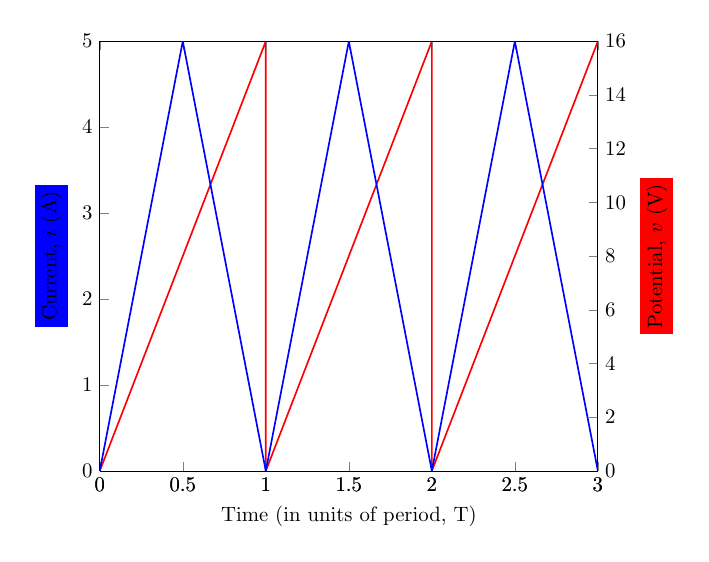
\begin{tikzpicture}[scale = 0.75]
      \pgfplotsset{
        scale only axis,
        xmin=0, xmax=3
      }
      \begin{axis}[
          axis y line*=right,
          ymin=0, ymax=16,
          xlabel={Time (in units of period, T)},
          ylabel={\colorbox{red}{Potential, $v$ (V)}},
        ]
        
        \addplot[thick,red]
        coordinates{
            (0,0)
            (1,16)
            (1,0)
            (2,16)
            (2,0)
            (3,16)
          };
      \end{axis}
      
      \begin{axis}[
          axis y line*=left,
          ymin=0, ymax=5,
          ylabel={\colorbox{blue}{Current, $i$ (A)}},
        ]
        
        \addplot[thick,blue]
        coordinates{
            (0,0)
            (0.5,5)
            (1,0)
            (1.5,5)
            (2,0)
            (2.5,5)
            (3,0)
          };
      \end{axis}
    \end{tikzpicture}
  \end{center}
  a) $\bar{v}(t)=\displaystyle{\frac{1}{T}\int_{0}^{T} v(t) \,dt=\frac{1}{\cancel{T}}\frac{1}{2}\cancel{T}\cdot16\volts}=\highlight{8\volts}$ \\
  $\bar{i}(t)=\displaystyle{\frac{1}{T}\int_{0}^{T} i(t) \,dt=\frac{1}{\cancel{T}}\frac{1}{2}\cancel{T}\cdot5\amps}=\highlight{2.5\amps}$ \\
  b) Voltage here can be expressed as a linear function $v(t)=\frac{16}{T}t$ for one period so \\
  $v_{rms}=\displaystyle{\sqrt{\frac{1}{T}\int_{0}^{T} v^2(t) \,dt}=\sqrt{\frac{1}{T}\frac{16^2}{T^2}\cdot\frac{T^3}{3}}=\frac{16\sqrt{3}}{3}}\approxeq\highlight{9.238\volts}$
  The same almost works for current $i(t)$ but it has to be made piecewise to account for the downward slope from $\displaystyle{\frac{T}{2}}$ to $T$, not that the sign really matters when doing the integration
  \[ i(t)=\begin{cases} 
      \frac{5}{T}t  & 0\leq t\leq \frac{T}{2} \\
      -\frac{5}{T}t & \frac{T}{2}\leq t\leq T \\
    \end{cases}
  \]
  which integrates as $i_{rms}=\displaystyle{\sqrt{\frac{1}{T}\left[\int_{0}^{\frac{T}{2}} i^2(t) \,dt+\int_{\frac{T}{2}}^{T} i^2(t) \,dt\right]}
    =\sqrt{\frac{1}{T}\frac{25}{T^2}\left[\frac{T^3}{6}+\frac{T^3}{3}-\frac{T^3}{24}\right]}
    =\sqrt{\frac{25}{\cancel{T^3}}\frac{8\cancel{T^3}}{24}}=\frac{5\sqrt{3}}{3}}\approxeq\highlight{2.887\amps}$\\
  c) $P_{avg}=v_{rms}i_{rms}=\highlight{26.67\watts}$
\end{soln}

% PROBLEM 3
\begin{problem}
Consider the following network of capacitors
\end{problem}
\begin{soln} ~\\
  \begin{center}
    \begin{circuitikz} \draw[scale = 1.5]
      (0,2) to[battery1, l_=$V_S\eq7\mathrm{V}$] (0,0) (0,2)
      to[capacitor, l=$C_1\eq1\mu\farad$] (2,2)
      to[capacitor, l=$C_3\eq3\mu\farad$] (4,2)
      to[capacitor, l=$C_4\eq6\mu\farad$] (4,0) -- (2,0)
      to[capacitor, l=$C_2\eq4\mu\farad$] (2,2) (2,0) -- (0,0)
      ;
    \end{circuitikz}
    \begin{circuitikz} \draw[scale = 1.5]
      (0,2) to[battery1, l_=$V_S\eq7\mathrm{V}$] (0,0) (0,2)
      to[capacitor, l=$C_{eq}\eq8.57\cdot10^{-7}\farad$] (2,2)
      -- (2,2)
      -- (2,0) -- (2,0) -- (0,0)
      ;
    \end{circuitikz}
  \end{center}
  a) Capacitor $C_{eq}$ must have a voltage drop of $7\volts$ to satisfy KVL therefore $Q_{tot}=C_{eq}V=6\mu\coulomb$. 
  Re-complicating the circuit and using $Q_{tot}$ we can find that the voltage drop across $C_1$ is $V_{C1}=\displaystyle{\frac{Q_{tot}}{C_1}}=6\volts$. By KVL
  this means that the rest of the circuit must contribute a potential drop of $1\volts$ which means that $C_2$ will experience a charge of $Q_{C2}=1\volts 4\mu\farad=4\mu\coulomb$
  therefore because charge is conserved the $C_3$-$C_4$ branch experiences the rest of $Q_{tot}$ or $Q_{C3C4}=Q_{tot}-Q_{C2}=2\mu\coulomb$. 
  Therefore the voltages across $C_3$ \& $C_4$ are $0.\bar{6}\volts$ \& $0.\bar{3}\volts$ respectively.
  \begin{center}
    \begin{tabular}{|l|l|l|}
      \hline Capacitor & Charge         & Voltage           \\\hline
      $C_1$            & $6\mu\coulomb$ & $6\volts$         \\
      $C_2$            & $4\mu\coulomb$ & $1\volts$         \\
      $C_3$            & $2\mu\coulomb$ & $0.\bar{6}\volts$ \\
      $C_4$            & $2\mu\coulomb$ & $0.\bar{3}\volts$ \\ \hline
    \end{tabular}
  \end{center}
  b) Once at equilibrium we would see a voltage drop across $C_1$ of $7\volts$ (so $Q=C_1V=7\mu\coulomb$) and no drop or charge across any other component because $C_1$, when fully charged,
  will act as a break in the circuit and not permit current to flow.
\end{soln}
\end{document}